\documentclass[11pt]{article}
\usepackage{arxiv}
\usepackage[utf8]{inputenc}
\usepackage[T1]{fontenc}
\usepackage{amsmath,amssymb,booktabs,graphicx,microtype,array,longtable}
\usepackage[colorlinks=true,allcolors=blue]{hyperref}
\usepackage{url}

\title{Query Anchoring Stabilizes Associative Retrieval\\Without Improving Classification:\\A Source-Bound Failure Analysis}
\author{Prepared for Ryan Gomez}
\date{20 October 2026}

\begin{document}
\maketitle

\begin{abstract}
Iterative associative retrieval can converge while degrading, preserving, or failing to improve a classifier. We study a narrow query-anchoring intervention motivated by a retained failure of an experimental EPU digit classifier. The intervention mixes the original query into every recurrent update, yielding a query-conditioned fixed point and a tractable displacement bound. We first identify a defect in a prior synthetic implementation: its purported unanchored recurrence multiplied retrieval by $0.1$ instead of using the required weight $1.0$. We preserve that evidence and introduce a corrected exploratory successor, V5. V5 separates mean, multi-prototype, and full-bank representations; compares direct and recurrent inference on identical banks; unit-normalizes the geometry; records 27,648 example-method outcomes; binds source and checkpoint hashes; and deterministically replays the complete result. Across known-mechanism simulations, multi-prototype representation resolves a constructed multimodal mean bottleneck (accuracy $1.000$ versus $0.497$), and anchoring reduces mean distractor displacement from $0.783$ to $0.077$. However, anchored top-$k$ recurrence gives exactly the same distractor accuracy as its direct same-bank control ($0.968$), failing the pre-specified one-point utility screen. The result supports a restricted conclusion: query anchoring controls movement, while the tested recurrence adds no predictive value beyond the representation on these simulations. The real EPU-QA1 digit study remains unexecuted because its frozen memory/pageout admission guard failed before data access. Accordingly, this paper is a complete negative-mechanism report, not a digit-efficacy, novelty, or submission-ready claim.
\end{abstract}

\section{Introduction}
Associative memories retrieve stored patterns from a query. Classical Hopfield networks formalized content-addressable computation through energy-based dynamics \cite{hopfield1982}; modern variants use continuous states and softmax retrieval closely related to attention \cite{ramsauer2020}. Convergence is useful only when the resulting state supports the task. A stable fixed point can preserve a wrong label, and a recurrent path can consume substantially more computation than direct retrieval while returning the same decision.

The EPU-QA1 line began from a retained empirical failure in which an iterative classifier underperformed a direct nearest-prototype control. Its original recurrence had no explicit query term in the stationary equation. We therefore ask a bounded question: does retaining the query in every update reduce destructive drift, and does that stability add predictive value over direct inference with the same memory bank?

The study separates two propositions. The mechanistic proposition is that anchoring reduces state displacement. The utility proposition is that this change improves classification beyond a same-bank direct decoder. This distinction is central: stability is neither correctness nor incremental utility.

Our contributions are:
\begin{enumerate}
  \item a complete contract for the query-anchored recurrence and its direct controls;
  \item discovery and repair of a prior implementation defect that invalidated the unanchored synthetic comparison;
  \item a factorial synthetic matrix that separates representation, recurrence, sparsity, and full-bank effects;
  \item immutable, source-bound records with deterministic replay and explicit negative outcomes; and
  \item a claim boundary that leaves real-data efficacy and population generalization unresolved.
\end{enumerate}

\section{Related work and novelty boundary}
Modern Hopfield networks establish continuous softmax retrieval, attention equivalence, and multiple attractor regimes \cite{ramsauer2020}. Universal Hopfield Networks decompose associative retrieval into similarity, separation, and projection, and show that alternative geometries can materially change performance \cite{millidge2022}. Encoded neural representations have also been proposed to improve separability and reduce metastable behavior \cite{kashyap2024}. These results make broad novelty claims for softmax recurrence, prototype retrieval, fixed context, or representation engineering indefensible here.

The contribution is therefore source-bound. We test whether a fixed query blend repairs a specific failure mode under a declared update. We do not claim that persistent inputs, sparse retrieval, continuous associative memory, or prototype banks are new. We also do not infer biological or hardware relevance.

\section{Problem formulation}
Let $M\in\mathbb{R}^{k\times d}$ contain memory rows $m_i$ with class labels $y_i$, and let $q\in\mathbb{R}^d$ be a unit-normalized query. Direct inference selects
\begin{equation}
  \hat\imath_0=\arg\max_i\langle m_i,q\rangle,
  \qquad \hat y_0=y_{\hat\imath_0},
\end{equation}
with deterministic bank-order tie breaking.

For inverse temperature $\beta>0$, define
\begin{equation}
  w_i(z)=\frac{\exp(\beta\langle m_i,z\rangle)}{\sum_j\exp(\beta\langle m_j,z\rangle)},
  \qquad r(z)=\sum_i w_i(z)m_i.
\end{equation}
The recurrent update is
\begin{equation}
  z_{t+1}=\alpha z_t+(1-\alpha)\left[(1-\lambda)q+\lambda r(z_t)\right],
  \qquad z_0=q. \label{eq:update}
\end{equation}
The original rule uses $\lambda=1$; the query-anchored candidate uses $\lambda=0.1$. Both use $\alpha=0.6$, $\beta=6$, and eight steps. Decoding applies the same bank and argmax rule to $z_8$.

The synthetic implementation uses unit-normalized rows. Consequently, dot-product and squared-Euclidean nearest-neighbor rankings agree, removing a geometry mismatch between direct and $k$-nearest-neighbor controls.

\section{Conditional analysis}
If $D=\max_{i,j}\|m_i-m_j\|$ and $L=\beta D^2/4$, the retrieval Jacobian has operator norm at most $L$. The recurrent map has Lipschitz constant
\begin{equation}
  c\leq\alpha+(1-\alpha)\lambda L.
\end{equation}
Thus $c<1$ is a sufficient contraction condition. This establishes a unique fixed point under the bound; it does not establish a correct label.

Because $z_0=q$ and both $q$ and each retrieved convex combination lie in the unit ball,
\begin{equation}
  \|z_t-q\|\leq 2\lambda(1-\alpha^t). \label{eq:displacement}
\end{equation}
Anchoring therefore directly limits movement. For memories $a$ and $b$, the score margin obeys
\begin{align}
\Delta_{t+1}={}&\alpha\Delta_t+(1-\alpha)(1-\lambda)\Delta_0\\
&+(1-\alpha)\lambda(m_a-m_b)^\top r(z_t).
\end{align}
The equation shows why the two propositions differ: a smaller movement can preserve an initial margin without improving whether that margin points to the correct class.

\section{Adversarial implementation audit}
The prior V4 synthetic runner labeled one method \texttt{original\_recurrent}, but its unanchored branch removed the query while retaining the candidate's retrieval coefficient $0.1$. It therefore computed
\[
z_{t+1}=\alpha z_t+(1-\alpha)0.1r(z_t)
\]
rather than the declared original update with $\lambda=1$. V4 remains historical evidence of the development process, but its comparison involving that method is invalid for the stated original recurrence.

V5 repairs this defect and adds three protections. First, every recurrent method receives an explicit \texttt{retrieval\_lambda}. Second, direct and recurrent comparisons share the exact same bank. Third, the run manifest binds all checkpoints and all executed source files, while the auditor verifies the full family-seed-example-method Cartesian product and reruns the experiment in a fresh temporary directory.

\section{Experimental design}
\subsection{Known-mechanism families}
Each seed creates disjoint training and test draws for two classes.
\begin{description}
  \item[Unimodal.] One mode per class; a class mean is sufficient.
  \item[Multimodal.] XOR-style class modes share nearly identical class means; a single mean is intentionally non-identifying.
  \item[Distractor.] Each class has a principal and boundary-adjacent mode, testing sensitivity to bank representation and recurrent movement.
\end{description}
These simulations are constructed diagnostics. They are not handwritten digits and cannot estimate deployment performance.

\subsection{Factorial method matrix}
The eight methods are direct mean, original mean recurrence, anchored mean recurrence, direct multi-prototype, original top-$k$ recurrence, anchored top-$k$ recurrence, direct full-bank retrieval, and three-neighbor full-bank voting. The mean bank stores one centroid per class; deterministic train-only spherical $k$-means builds two prototypes per class; the full bank stores every training row. This matrix isolates representation from recurrence. Score-evaluation counts expose computation differences.

\subsection{Frozen V5 checks}
V5 was designed after V1--V4 were inspected, so it is exploratory even though its four checks were serialized before V5 execution. The checks require: a $0.25$ multimodal accuracy gain from multi-prototype over mean direct retrieval; a $0.10$ distractor displacement reduction from anchoring; a $0.01$ distractor accuracy gain from anchored top-$k$ recurrence over direct multi-prototype retrieval; and a $0.05$ distractor accuracy gain from three-neighbor voting over direct multi-prototype retrieval.

Eight fixed random streams are used as simulation replications. We report means, standard deviations, and ranges; they are not treated as human-writer clusters or as a basis for population significance claims.

\section{Results}
% Generated from the audited V5 aggregate.
\begin{table*}[t]
\centering
\scriptsize
\setlength{\tabcolsep}{3.5pt}
\caption{V5 exploratory synthetic results. Accuracy, mean query displacement, prediction-change rate, and score evaluations are means across eight simulation seeds.}
\label{tab:v5-results}
\begin{tabular}{llrrrr}
\toprule
Family & Method & Accuracy & Displacement & Changed & Score evals \\
\midrule
distractor & direct\_mean & 0.959 & 0.000 & 0.000 & 2 \\
distractor & original\_mean & 0.959 & 0.783 & 0.000 & 18 \\
distractor & anchor\_mean & 0.959 & 0.077 & 0.000 & 18 \\
distractor & direct\_multi & 0.968 & 0.000 & 0.000 & 4 \\
distractor & original\_topk & 0.968 & 0.241 & 0.000 & 36 \\
distractor & anchor\_topk & 0.968 & 0.020 & 0.000 & 36 \\
distractor & direct\_full & 0.961 & 0.000 & 0.000 & 96 \\
distractor & knn & 0.977 & 0.000 & 0.000 & 96 \\
\midrule
multimodal & direct\_mean & 0.497 & 0.000 & 0.000 & 2 \\
multimodal & original\_mean & 0.497 & 0.896 & 0.000 & 18 \\
multimodal & anchor\_mean & 0.497 & 0.087 & 0.000 & 18 \\
multimodal & direct\_multi & 1.000 & 0.000 & 0.000 & 4 \\
multimodal & original\_topk & 1.000 & 0.140 & 0.000 & 36 \\
multimodal & anchor\_topk & 1.000 & 0.013 & 0.000 & 36 \\
multimodal & direct\_full & 1.000 & 0.000 & 0.000 & 96 \\
multimodal & knn & 1.000 & 0.000 & 0.000 & 96 \\
\midrule
unimodal & direct\_mean & 1.000 & 0.000 & 0.000 & 2 \\
unimodal & original\_mean & 1.000 & 0.188 & 0.000 & 18 \\
unimodal & anchor\_mean & 1.000 & 0.019 & 0.000 & 18 \\
unimodal & direct\_multi & 1.000 & 0.000 & 0.000 & 4 \\
unimodal & original\_topk & 1.000 & 0.191 & 0.000 & 36 \\
unimodal & anchor\_topk & 1.000 & 0.016 & 0.000 & 36 \\
unimodal & direct\_full & 1.000 & 0.000 & 0.000 & 96 \\
unimodal & knn & 1.000 & 0.000 & 0.000 & 96 \\
\bottomrule
\end{tabular}
\end{table*}

% Generated from the audited V5 hypothesis outcomes.
\begin{table}[t]
\centering
\small
\caption{V5 checks fixed before V5 execution. V5 was informed by V1--V4 and remains exploratory.}
\label{tab:v5-hypotheses}
\begin{tabular}{lrrl}
\toprule
Check & Required & Observed & Status \\
\midrule
REPRESENTATION & 0.250 & 0.503 & PASS \\
ANCHOR-STABILITY & 0.100 & 0.706 & PASS \\
RECURRENT-UTILITY & 0.010 & 0.000 & FAIL \\
FULL-BANK & 0.050 & 0.010 & FAIL \\
\bottomrule
\end{tabular}
\end{table}


\begin{figure*}[t]
  \centering
  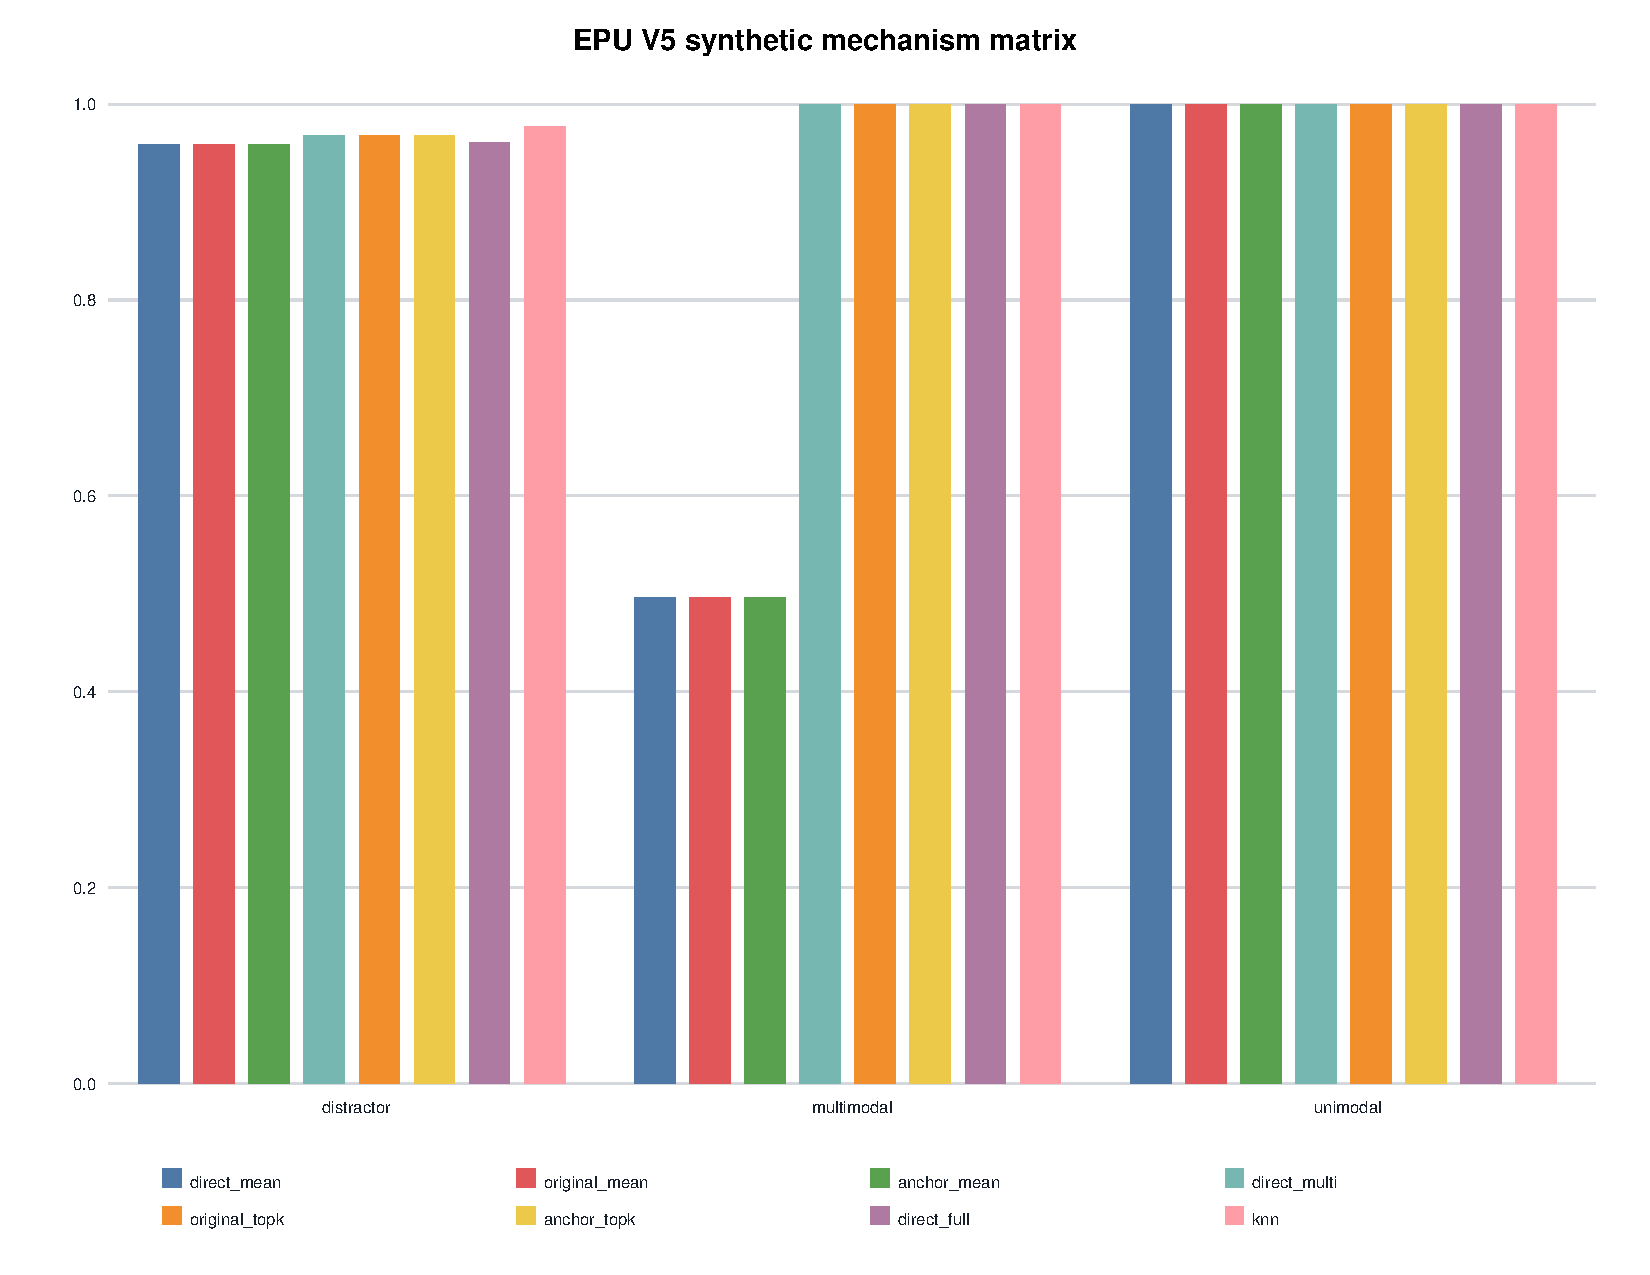
\includegraphics[width=0.96\textwidth]{generated/v5_accuracy.pdf}
  \caption{Mean accuracy across eight V5 simulation seeds. Recurrent variants do not exceed their same-bank direct controls in these families.}
  \label{fig:v5-accuracy}
\end{figure*}

V5 retained 27,648 example-method records. The multi-prototype direct method achieved $1.000$ on the constructed multimodal family versus $0.497$ for the direct class-mean method, passing the representation check by $0.503$. This is expected evidence that the construction actually exposes the intended representation bottleneck.

On the distractor family, the original mean recurrence moved $0.783$ on average, whereas the anchored mean recurrence moved $0.077$, passing the stability check by $0.706$. Both produced the same accuracy as direct mean retrieval, $0.959$, and neither changed any predicted class.

The central utility screen failed. Anchored top-$k$ recurrence and its direct multi-prototype control both reached $0.968$, for an observed difference of exactly $0.000$ against a required $0.010$. The recurrence used nine times as many score evaluations (36 versus 4). Three-neighbor voting reached $0.977$ but improved by only $0.010$, failing its deliberately stronger $0.050$ screen.

The result is scientifically useful because it discriminates mechanisms. Representation changes solve the deliberately constructed multimodal failure. Anchoring strongly controls trajectory displacement. The tested recurrence adds no classification value beyond its representation.

\section{Real-data protocol and blocked execution}
The frozen EPU-QA1 development protocol targets the scikit-learn 1,797-row subset of the UCI Optical Recognition of Handwritten Digits data. The full UCI resource contains 5,620 64-feature instances and documents disjoint writers in its official training and test sets \cite{uci1998}. The locally installed subset does not expose writer identifiers, so it cannot support writer-level independence.

The E5-R1 controller requires 31 resource samples over at least 30 seconds with at least 1 GiB free-plus-speculative memory before reserving the sole replacement attempt, plus a 512 MiB runtime floor and stable pageouts. The latest retained attempt was refused before data access. The current host remained below the floor during this work, so the replacement attempt was not spent. Synthetic results cannot replace this missing execution.

\section{Threats to validity and limitations}
The synthetic generators encode the mechanisms they test. Their positive representation result is therefore a construction check, not a discovery about natural data. V5 was informed by earlier phases and is exploratory. The seed count is small, and the random streams are not independent people, devices, or acquisition sites. No learned encoder, calibration study, probability model, adversarial perturbation suite, or real OOD domain is evaluated.

The multi-prototype fit uses deterministic spherical $k$-means and thus adds representational capacity. V5 controls this by comparing direct and recurrent inference on the same bank, but it does not equalize storage with the mean bank. Full-bank methods use more memory. Score evaluations are an implementation-independent cost proxy, not a hardware energy measurement.

The proof bounds are conditional and may be loose. Contraction, energy decrease, and small displacement cannot imply classification accuracy. The present work does not establish architecture novelty, state of the art, digit efficacy, population generalization, biological plausibility, or hardware efficiency.

\section{Reproducibility and evidence integrity}
The V5 configuration, raw JSONL records, per-seed CSV, per-cell checkpoints, aggregates, hypotheses, report, figure, and audit are retained under a single run directory. The manifest binds the executed Python sources and every checkpoint. The auditor verifies 27,648 unique Cartesian cells, recomputes aggregates and hypothesis outcomes, verifies report hashes, and performs a byte-level deterministic replay of the scientific outputs. The claim-evidence matrix maps each manuscript claim to its artifact and disposition.

Reproduction remains same-host engineering verification. Independent reproduction requires another executor and environment, and has not occurred.

\section{Discussion}
The study illustrates a common evaluation error: an intervention can repair a mathematical property without repairing the task. Query anchoring changes the fixed-point equation and reduces drift, but the direct decoder already contains the relevant decision on these geometries. Repeated retrieval then consumes more score evaluations without adding information. When the class mean is insufficient, changing representation matters; recurrence over an insufficient bank does not create the missing modes.

The next defensible real-data study should retain same-bank direct controls, writer-disjoint groups, a predeclared practical effect threshold that includes compute cost, and a new protocol frozen before protected outcomes. If the direct comparator remains equal or stronger, the utility branch should close rather than searching adaptively for a favorable configuration.

\section{Conclusion}
Query anchoring is an effective movement constraint in the tested synthetic systems, but it does not improve classification over direct inference with the same memory bank. A corrected and fully audited successor therefore yields a mixed mechanistic result and a negative utility result. The evidence supports continued use of direct inference as the default for these synthetic families. EPU-QA1 remains incomplete on real digits because the frozen development run has not passed resource admission, and no confirmatory or independently reproduced result exists.

\bibliographystyle{plain}
\bibliography{references}

\appendix
\section{Artifact lineage}
The local \texttt{arxiv.sty} is a project-specific adaptation of the user's existing local style shim. Only its header text and package date were adapted for this manuscript. The scientific assets are generated only after the V5 adversarial audit passes.

\section{Disposition vocabulary}
Engineering verification means that code and artifact contracts passed. Exploratory synthetic pass or fail refers only to a V5 check. \texttt{BLOCKED\_RESOURCE} means the guarded real-data attempt refused before opening its payload. None of these states implies confirmation, independent reproduction, submission, or publication.

\end{document}
